\documentclass[journal,12pt,twocolumn]{IEEEtran}

\usepackage{setspace}
\usepackage{gensymb}

\singlespacing


\usepackage[cmex10]{amsmath}

\usepackage{amsthm}

\usepackage{mathrsfs}
\usepackage{txfonts}
\usepackage{stfloats}
\usepackage{bm}
\usepackage{cite}
\usepackage{cases}
\usepackage{subfig}

\usepackage{longtable}
\usepackage{multirow}

\usepackage{enumitem}
\usepackage{mathtools}
\usepackage{steinmetz}
\usepackage{tikz}
\usepackage{circuitikz}
\usepackage{verbatim}
\usepackage{tfrupee}
\usepackage[breaklinks=true]{hyperref}
\usepackage{graphicx}
\usepackage{tkz-euclide}
\usepackage{float}

\usetikzlibrary{calc,math}
\usepackage{listings}
    \usepackage{color}                                            %%
    \usepackage{array}                                            %%
    \usepackage{longtable}                                        %%
    \usepackage{calc}                                             %%
    \usepackage{multirow}                                         %%
    \usepackage{hhline}                                           %%
    \usepackage{ifthen}                                           %%
    \usepackage{lscape}     
\usepackage{multicol}
\usepackage{chngcntr}

\DeclareMathOperator*{\Res}{Res}

\renewcommand\thesection{\arabic{section}}
\renewcommand\thesubsection{\thesection.\arabic{subsection}}
\renewcommand\thesubsubsection{\thesubsection.\arabic{subsubsection}}

\renewcommand\thesectiondis{\arabic{section}}
\renewcommand\thesubsectiondis{\thesectiondis.\arabic{subsection}}
\renewcommand\thesubsubsectiondis{\thesubsectiondis.\arabic{subsubsection}}


\hyphenation{op-tical net-works semi-conduc-tor}
\def\inputGnumericTable{}                                 %%

\lstset{
%language=C,
frame=single, 
breaklines=true,
columns=fullflexible
}
\begin{document}


\newtheorem{theorem}{Theorem}[section]
\newtheorem{problem}{Problem}
\newtheorem{proposition}{Proposition}[section]
\newtheorem{lemma}{Lemma}[section]
\newtheorem{corollary}[theorem]{Corollary}
\newtheorem{example}{Example}[section]
\newtheorem{definition}[problem]{Definition}

\newcommand{\BEQA}{\begin{eqnarray}}
\newcommand{\EEQA}{\end{eqnarray}}
\newcommand{\define}{\stackrel{\triangle}{=}}
\bibliographystyle{IEEEtran}
\providecommand{\mbf}{\mathbf}
\providecommand{\pr}[1]{\ensuremath{\Pr\left(#1\right)}}
\providecommand{\qfunc}[1]{\ensuremath{Q\left(#1\right)}}
\providecommand{\sbrak}[1]{\ensuremath{{}\left[#1\right]}}
\providecommand{\lsbrak}[1]{\ensuremath{{}\left[#1\right.}}
\providecommand{\rsbrak}[1]{\ensuremath{{}\left.#1\right]}}
\providecommand{\brak}[1]{\ensuremath{\left(#1\right)}}
\providecommand{\lbrak}[1]{\ensuremath{\left(#1\right.}}
\providecommand{\rbrak}[1]{\ensuremath{\left.#1\right)}}
\providecommand{\cbrak}[1]{\ensuremath{\left\{#1\right\}}}
\providecommand{\lcbrak}[1]{\ensuremath{\left\{#1\right.}}
\providecommand{\rcbrak}[1]{\ensuremath{\left.#1\right\}}}
\theoremstyle{remark}
\newtheorem{rem}{Remark}
\newcommand{\sgn}{\mathop{\mathrm{sgn}}}
\providecommand{\abs}[1]{\lvert#1\vert}
\providecommand{\res}[1]{\Res\displaylimits_{#1}} 
\providecommand{\norm}[1]{\lVert#1\rVert}
%\providecommand{\norm}[1]{\lVert#1\rVert}
\providecommand{\mtx}[1]{\mathbf{#1}}
\providecommand{\mean}[1]{E[ #1 ]}
\providecommand{\fourier}{\overset{\mathcal{F}}{ \rightleftharpoons}}
%\providecommand{\hilbert}{\overset{\mathcal{H}}{ \rightleftharpoons}}
\providecommand{\system}{\overset{\mathcal{H}}{ \longleftrightarrow}}
	%\newcommand{\solution}[2]{\textbf{Solution:}{#1}}
\newcommand{\solution}{\noindent \textbf{Solution: }}
\newcommand{\cosec}{\,\text{cosec}\,}
\providecommand{\dec}[2]{\ensuremath{\overset{#1}{\underset{#2}{\gtrless}}}}
\newcommand{\myvec}[1]{\ensuremath{\begin{pmatrix}#1\end{pmatrix}}}
\newcommand{\mydet}[1]{\ensuremath{\begin{vmatrix}#1\end{vmatrix}}}
\numberwithin{equation}{subsection}
\makeatletter
\@addtoreset{figure}{problem}
\makeatother
\let\StandardTheFigure\thefigure
\let\vec\mathbf
\renewcommand{\thefigure}{\theproblem}
\def\putbox#1#2#3{\makebox[0in][l]{\makebox[#1][l]{}\raisebox{\baselineskip}[0in][0in]{\raisebox{#2}[0in][0in]{#3}}}}
     \def\rightbox#1{\makebox[0in][r]{#1}}
     \def\centbox#1{\makebox[0in]{#1}}
     \def\topbox#1{\raisebox{-\baselineskip}[0in][0in]{#1}}
     \def\midbox#1{\raisebox{-0.5\baselineskip}[0in][0in]{#1}}
\vspace{3cm}
\title{Assignment 3}
\author{Satya Sangram Mishra}
\maketitle
\newpage
\bigskip
\renewcommand{\thefigure}{\theenumi}
\renewcommand{\thetable}{\theenumi}
Download all python codes from 
\begin{lstlisting}
https://github.com/satyasm45/Summer-Internship/tree/main/Assignment-3/Codes
\end{lstlisting}
%
and latex-tikz codes from 
%
\begin{lstlisting}
https://github.com/satyasm45/Summer-Internship/tree/main/Assignment-3
\end{lstlisting}
%
\section{Question No. 2.55}
Let $\vec{A}$ and $\vec{B}$ be the centres of two circles
of equal radii 3 such that each one of them
passes through the centre of the other. Let them
intersect at $\vec{C}$ and $\vec{D}$. Is AB$\perp$CD?
%
\section{Solution}
To perform the given construction let us assume 
\begin{align}
\vec{A}=\myvec{0\\0}
\end{align}

Based on the constraints given in the question, $\vec{B}$ will lie on the circle with center as $\vec{A}$ and radius 3.Without loss of generality,let us assume:
\begin{align}
\vec{B}=\myvec{3\\0}
\end{align}
Then,
\begin{align}
\norm{\vec{B}-\vec{A}} = \norm{\vec{A}-\vec{B}}=\norm{\vec{B}}  = 3 \quad \brak{\because \vec{A}=0}
\end{align}
The centers and radii of the two circles are now given in table \ref{tab:table1}
\numberwithin{table}{section}
\begin{table}[!ht]
\begin{center}
\begin{tabular}{ | m{2cm} | m{2cm} | m{2cm} |} 
\hline
 & Circle 1 & Circle 2 \\
\hline
Centre  & $\vec{A}$=\myvec{0\\0} & $\vec{B}$=\myvec{3\\0} \\ 
\hline
Radius & $r_{1}$=3 &$r_{2}$=3  \\ 
\hline
\end{tabular}
\end{center}
\caption{Input values}
\label{tab:table1}

\end{table}

Let us define:
\begin{align}
\vec{u}=\myvec{\cos \theta\\  \sin \theta},  \theta \in [0,2\pi].
\end{align}

Then any point \myvec{x_{1}\\y_{1}} on Circle 1 is given by :
\begin{align}
\myvec{x_{1}\\y_{1}}=\vec{A}+r_{1}\vec{u}=3\myvec{\cos \theta\\ \sin \theta}\quad \brak{\because \vec{A}=0}
\end{align}

 This is the locus of Circle 1.

Similarly,locus of Circle 2 is given by:
\begin{align}
\myvec{x_{2}\\y_{2}}=\vec{B}+r_{2}\vec{u}=\myvec{3\\0}+3\myvec{\cos\theta\\  \sin \theta}
\end{align}

Using the locus of the circles Fig. \ref{fig:circle} was plotted.

\numberwithin{figure}{section}
\begin{figure}[H]
\centering
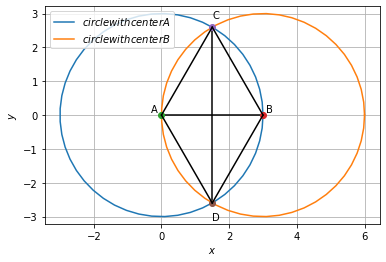
\includegraphics[width=\columnwidth]{figure3}
\caption{Circles with their points of intersection}
\label{fig:circle}	
\end{figure}

We have $\vec{C}$ and $\vec{D}$ as points of intersection.So,

\begin{align}
\norm{\vec{D}-\vec{A}} = \norm{\vec{C}-\vec{A}}=r_{1}=3
\end{align}

\begin{align}
\norm{\vec{D}-\vec{B}} = \norm{\vec{C}-\vec{B}}=r_{2}=3
\end{align}
Therefore,in quadrilateral ACBD we have
\begin{align}
\norm{\vec{D}-\vec{B}} = \norm{\vec{C}-\vec{B}}=\norm{\vec{D}-\vec{A}} = \norm{\vec{C}-\vec{A}}=3 \label{eq:0}
\end{align}

So,ACBD is a Rhombus.
For a Rhombus we have diagonals bisect each other at right angles.

Therefore it can be concluded that AB$\perp$CD.

We can also verify the result by using equation \ref{eq:0} and doing some compuatations:
\begin{align}
\norm{\vec{C}-\vec{A}}^2 = \norm{\vec{C}-\vec{B}}^2
\end{align}
Also, $\norm{\vec{P}}^2=\vec{P}^T\vec{P}$ .So,
\begin{align}
(\vec{C}-\vec{A})^T(\vec{C}-\vec{A})=(\vec{C}-\vec{B})^T(\vec{C}-\vec{B})
\\
\implies \vec{A}^T\vec{C}-\vec{B}^T\vec{C}=\vec{C}^T\vec{B}-\vec{C}^T\vec{A}+\norm{\vec{A}}^2-\norm{\vec{B}}^2 
\end{align}
For any two vectors $\vec{P}$ and $\vec{Q}$ we have 

$\vec{P}^T\vec{Q}=\vec{Q}^T\vec{P}$.So,
\begin{align}
2\times \vec{A}^T\vec{C}-2\times\vec{B}^T\vec{C}=\norm{\vec{A}}^2-\norm{\vec{B}}^2 \label{eq:1}
\end{align}
Similarly,using:
\begin{align}
\norm{\vec{D}-\vec{A}}^2 = \norm{\vec{D}-\vec{B}}^2
\end{align}
We get:
\begin{align}
2\times \vec{A}^T\vec{D}-2\times\vec{B}^T\vec{D}=\norm{\vec{A}}^2-\norm{\vec{B}}^2 \label{eq:2}
\end{align}

Subtracting equation \ref{eq:2} from equation \ref{eq:1}:
\begin{align}
2\times(\vec{A}^T-\vec{B}^T)(\vec{C}-\vec{D})=0
\\
\implies (\vec{A}-\vec{B})^T(\vec{C}-\vec{D})=0
\\
\implies AB\perp CD
\end{align}
\end{document}